\section{Bayesian Filtering}
\subsection{Overview}

This section will introduce and describe the Bayesian for solving time-dependent inverse problems, laying out the theoretical foundations of the taken approach. In Section 2.3 we reformulate the definition of inverse problems for the finite-dimensional time-dependent case. We then present the pendulum problem, which will be studied along the whole thesis to illustrate important ideas. In Section 2.4 we present first present the classical approach for solving inverse problems and the challenges it encounters with noisy data. We next present the Bayesian approach, and show how it incorporates prior information about the structure of the problem to address uncertainty. We then adapt the definition of the pendulum problem to the Bayesian framework. Finally, Section 2.5 presents important results, including a characterization of the class of well-posed inverse problems. We conclude the section by proving that the pendulum problem is well-posed.

\subsection{Set-Up}

We study parametrized models for which the value of the \textit{parameter} $u \in X$ is unknown or uncertain. To model the behaviour of the system, we introduce \textit{forward response operators} $\mathcal{G} : X \rightarrow Y$ mapping values of the \textit{parameter space} to the \textit{data space}, assuming both spaces to be finite-dimensional vector spaces.

We consider a real system described by $\mathcal{G}$ and the true parameter $u^* \in X$, and assume that \textit{observations} $y_{obs} \in Y$ of the system are available from measurements. The data $y$ is then the image of the true parameter under the mapping $\mathcal{G}$. Due to noise present in the data, we obtain the following approximate model

\begin{equation}\label{inverse-formula}
  y_{obs} \approx \G(u^*),
\end{equation}

and the question \textit{To which extent can we find the \textit{inverse} of the data $y_{obs}$ under the forward response operator $\G$?} Answering this question is known as the \textit{inverse problem}.

In this thesis, we are interested in solving the inverse problem by incrementaly building up knowledge about the unknown. To do this, we decompose the data and consider a growing sequence of observations made available for analysis. The advantages of this approach are twofold. First, it allows to perform inference on running dynamical systems and update our knowledge as more measurements become available. Second, it can also be used for non-dynamical problems in the hope to transform one hard problem in a sequence of smaller problems that can hopefully be solved more efficiently.

In this sequential formulation, the data $y$ is decomposed in a finite sequence of observations $y_{obs} = (y_{obs}^{(1)}, \ldots, y_{obs}^{(N)})$ \note{maybe it's relevant to cite \cite{chopin_2002} here}. We also decompose the forward response oeprator $\G$ in a sequence of operators $\{\G_i\}_{i=1}^N$ such that

\begin{equation*}
  y_{obs}^{(i)}\approx \G_i(u^*).
\end{equation*}


This allows us to reformulate the question from above as \textit{How can we use new observations to update our knowledge about $\theta_{true}$?} Answering this new question is called the \textit{filtering problem}, and solving inserve and filtering problems will be the focus of this thesis.

One situation where this decomposition can naturally be used is when the system is described by a initial value problem of the form

\begin{equation}
  \begin{aligned}
    \frac{\text{d}x}{\text{d}t} &= f(x; u^*)\\
    x(0) &= x_0,
  \end{aligned}
\end{equation}  

where $u^* \in X$ is the parameter of the model, and the solution $x(t; u^*)$ is assumed to exist for every time $t \geq 0$. The sequence of observations then correspond to measurements at times  $0 \leq t_1 < \ldots < t_N$. We further use an \textit{observational operator} $\mathcal{O}$ to model the measurement procedure, mapping states of the system to observations. The sequence of forward response operator is $\G_i : X \rightarrow Y$ are then given by $\G_i = \mathcal{O} \circ x(t_i; \cdot)$. We illustrate this in the next section.

\subsection{Pendulum problem}

We now introduce a filtering problem that will guide the rest of the thesis. Using a pendulum, we would like to estimate the value of the Earth's gravitational acceleration. To do this, we first had to model the behaviour of the pendulum using a model parametrized by the gravitational acceleration $g$. We chose to use the \textit{simple pendulum model}, a simplified model that ignores the mass of the hanging mass and of the string, ignores the forces of friction present on the hanging mass and assumes the movement on the pendulum is only happening on one plane. This model is illustrated in Figure 1. This simplification allows to model the state of the pendulum with a single value $x(t)$ representing the angle of the pendulum to the resting point, described by the following differential equation

\begin{equation}\label{pendulum-ode}
  \frac{\text{d}^2x}{\text{d}t^2} = -\frac{g}{l}\sin(x).
\end{equation}

In this model, $g$ is the Earth's gravitational acceleration and $l$ is the length of the string holding the hanging mass.

We proceeded to run an experiment, in which the pendulum was let go from an initial angle of $5^\circ$ and no initial velocity. We then measured the first $N = 9$ times at which the pendulum was aligned with the vertical axis, indicating a null angle.

\subsection{Bayesian filtering}

The previous paragraphs focused on giving a definition of inverse and filtering problems. Before starting to discuss solutions to these problems, we present the concept of \textit{well-posedness} first given by Hadamard for describing properties of models of physical phenomena.

\begin{definition} A problem is said to be \textit{well-posed} if it satisfies the following conditions:
  \begin{enumerate}
  \item{a solution exists,}
  \item{the solution is unique,}
  \item{the solution changes continuously with the initial condition.}
  \end{enumerate}

  A problem failing to satisfy these conditions is said to be \textit{ill-posed}. In the context of inverse problems, the 3rd property should be understand as continuity of the solution of the problem with respect to the data.  
\end{definition}

A possible way to solve inverse problems is to try to find a value $u^* \in X$ that solves the inverse problem \textit{as well as possible}. This is done by replacing the inverse problem by the optimization problem

\begin{equation*}
  u^* = \underset{u \in X}{\text{argmin}} \norm{ y_{obs} - \G(u) }_Y.
\end{equation*}

However, finding a global minimum in the presence of noise is often a difficult task since it might not exist, or the minimized function might admit multiple local minima. Solving the inverse problem by minimization is thus an ill-posed problem. While some of these difficulties can be addresses by \textit{regularization}, two issues remain unresolved. First, regularization and the choice of the minimized norm are \textit{ad hoc} decisions that are not part of the modelling process. Then, assuming that the optimization algorithm does provide an estimate $\hat u$, this point estimate does not contain information about the quality, or \textit{uncertainty}, of this estimation. We chose to study a different approach for solving inverse problems: the Bayesian framework.

\note{maybe skip the bitching?}

In the Bayesian framework, the model is not anymore treated as an equation that has to be inverted, but rather as an encoding the relation between the knowns and the unknowns of the system. In this encoding, we represent every variable using \textit{random variables} and refine the model to include every available information of the system. This allows us to rewrite the standard inverse problem as follows

\begin{equation}
  y = \G(u) + \eta.
\end{equation}

Here, the variable $y$ models the measurements of the system, and the observations $y_{obs}$ are treated as realizations of this random variable. Existing knowledge about the parameter \textit{prior} collecting the data is incorporated in the distribution of $u$, called the \textit{prior distribution} with measure $\mu_0$. The remaining variable $\eta$ is used to represents the uncertainty in the observations $y$. Commonly, $\eta$ is used to incorporate measurement noise or modelling error, and is often model using a mean-zero Gaussian distribution.

The coupling of these random variables allows to answer a wide range of questions about the model through the use of conditioning. For instance, in a situation where the real parameter $u = u^*$ is known, we can consider the conditioned random variable $y|u$. The probability density of this conditioned random variable is refered to as the \textit{likelihood function}. If  $\rho$ denotes the density function of $\eta$, the likelihood function is

\begin{equation}\label{def-ell}
  \ell(y|u) := \rho(y - \G(u)).
\end{equation}
\note{maybe extend this to filtering and sequence of likelihoods}

Motivated by the wide use of the Gaussian distribution for error modelling, we assume throughout the thesis that the likelihood function can be written as

\begin{equation} \label{exponential-ell}
  \ell(y|u) = \exp(-\Phi(u;y)),
\end{equation}

where $\Phi$ is called a \textit{potential function}, or \textit{negative log-likelihood}. In the case where the uncertainty is modeled by a multivariate Gaussian distribution $\eta \sim \mathcal{N}(0, \Gamma)$, the potential function is given by

\begin{equation} \label{gaussian-potential}
  \Phi(u; y) = \norm{\Gamma^{-1/2}(y - \G(u))}_Y^2.
\end{equation}
\note{reference to the link between regularization and error modelling? }


When solving the inverse problem, we are interested in learning how observed data update our prior believes about the model's parameters. This question can be naturally translated into studying the conditional distribution of $u$ under the observations $y = y_{obs}$. The new knowledge about the parameter $u$ is then contained in the distribution of $u|y$, called the \textit{posterior distribution} with measure $\mu^y$. Intuitively, \textit{Bayes' rule} can be used to find the posterior distribution in terms of the prior distribution and the likelihood.

Given a probability triplet $(\Omega, \mathcal{F}, \P)$, and two events $A, B \in \mathcal{F}$ with $\P(B) > 0$, Bayes' rule gives the distribution of the conditioned event $\P(A|B)$ by

\begin{equation*}
  \P(A|B) = \frac{\P(B|A)\P(A)}{P(B)}.
\end{equation*}

An informal extension of this theorem to infinitesimal events gives the following relation for the posterior distribution

\begin{equation*}\label{bayes-rule}
  \mu^y(\text{d}u) \propto \ell(y|u)\mu_0(\d u),
\end{equation*}

where the $\propto$ symbol denotes proportionality up to a constant factor. This framework for solving inverse problems can be used to express filtering problems, and thus also provide a solution to the later. 

\note{TODO: extend to filtering and show two examples of sequences of likelihoods and their intermediate updates}

While this argument does provide the correct result, the extension of Bayes' rule from events to probability measures is not valid. Moreover, it is not clear which assumptions are made about the model to ensure existence  the solution, and more generally, well-posedness has not been discussed. A more rigorous proof and characterization of well-posed inverse problems will now be presented.

We start by stating the following assumptions

\begin{assumption}\label{assumption-ll}
  The function $\Phi : X \times Y \rightarrow \mathbb{R}$ has the following properties.
  
  \begin{enumerate}
  \item For every $\epsilon > 0$ and $r > 0$ there is an $M \in \mathbb{R}$ such that, for all $u \in X$ and all $y \in Y$ with $\norm{y}_Y < r$,
    \begin{equation*}
      \Phi(u; y) \ge M - \epsilon\norm{u}_X^2.
    \end{equation*}
  \item For every $r > 0$ there is a $K > 0$ such that, for all $u \in X$ and $y \in Y$ with $\text{max}\{\norm{u}_X, \norm{y}_Y\} < r$,
    \begin{equation*}
      \Phi(u; y) \le K.
    \end{equation*}

  \item For every $r > 0$ there is a $L > 0$ such that, for all $u_1, u_2 \in X$ and $y \in Y$ with $\text{max}\{\norm{u_1}_X, \norm{u_2}_X, \norm{y}_Y\} < r$,

    \begin{equation*}
      |\Phi(u_1; y) - \Phi(u_2; y)| \le L\norm{u_1 - u_2}_X.
    \end{equation*}

  \item For every $\epsilon > 0$ and $r > 0$ there is a $C \in \mathbb{R}$ such that, for all $y_1, y_2 \in Y$ with $\text{max}\{\norm{y_1}_Y, \norm{y_2}_Y\} < r$, and for all $u \in X$,

    \begin{equation*}
      |\Phi(u; y_1) - \Phi(u; y_2)| \le \exp(\epsilon\norm{u}_X^2 + C)\norm{y_1 - y_2}_Y.
    \end{equation*}
  \end{enumerate}
\end{assumption}

These mild assumptions happen to be rather easy to fulfill for many practical problems. They provide with upper and lower bounds, and Lipshitz continuity with respect to the data $y$ and the parameter $u$.  However, since potential functions often are of the form of (\ref{gaussian-potential}), we are interested in refining these assumptions to the shared structure of such problems.

\begin{assumption}\label{assumption-fw}
  The function $\G : X \rightarrow \mathbb{R}^N$ has the following properties.

  \begin{enumerate}
  \item For every $\epsilon > 0$ there is an $M \in \mathbb{R}$ such that for all $u \in X$,
    \begin{equation*}
      |\G(u)|_\Gamma \le \exp(\epsilon \norm{u}_X^2 + M).
    \end{equation*}
  \item For every $r > 0$ there is a $K > 0$ such that, for all $u_1, u_2 \in X$ with $\text{max}\{\norm{u_1}_X, \norm{u_2}_X\} < r$,
    \begin{equation*}
      |\G(u_1) - \G(u_2)|_\Gamma \le K\norm{u_1 - u_2}_X.
    \end{equation*}
  \end{enumerate}
\end{assumption}

We can naturally use these assumptions on the forward response operator $\G$ to derive properties of the potential function using the following lemma.

\begin{lemma} \label{fw-implies-ll}
  Assume that $\G  : X \rightarrow \mathbb{R}^N$ satisfies Assumption \ref{assumption-fw}. Then, for any covariance matrix $\Gamma$, the potential function given by (\ref{gaussian-potential}) satisfies Assumption \ref{assumption-ll} with $(Y, \norm{\cdot}_Y) = (\mathbb{R}^N, \norm{\cdot}_\Gamma)$.
\end{lemma}

\begin{proof} \note{This is trivial, can I skip this proof?}
\end{proof}

Using these assumptions, we can now proceed to provide a formal proof of Bayes' rule for continuous random variables and (\ref{bayes-rule}). The following theorem will play a central role in proving

\begin{theorem}
  \label{duley}
  Let $\mu, \nu$ be probability measures on $S \times T$, where $(S, \mathcal{A})$ and $(T, \mathcal{B})$ are measurable spaces. Let $(x, y) \in S \times T$. Assume that $\mu \ll \nu$ and that $\mu$ has Radon-Nikodym derivative $\phi$ with respect to $\mu$. Assume further that the conditional distributions of $x|y$ under $\nu$, denoted by $\nu^y(\d x)$, exists. Then the conditional distribution of $x|y$ under $\mu$, denoted $\mu^y(\d x)$, exists and $\mu^y(\d x) \ll \nu^y(\d x)$. The Radon-Nikodym derivative is given by

  \begin{equation}
    \frac{\d \nu^y}{\d \mu^y}(x) =  \begin{cases}
      \frac1{c(y)}\phi(x,y) & \text{if $c(y) > 0$, and}\\
      1 & \text{else,}
    \end{cases}  
  \end{equation}

  where $c(y) = \int_{S}\phi(x,y)\d \mu^y(x)$ for all $y \in T$.
\end{theorem}

\begin{proof}
  The proof of this theorem is given by Dudley \cite{dudley_2002}.
\end{proof}

We now state Bayes' rule for continuous distribution and prove it using the previously stated theorem.

\begin{theorem}[Generalized Bayes' Rule]
  Assume that the likelihood function is given as in (\ref{exponential-ell}) where $\Phi$ satisfies Assumptions \ref{assumption-ll} and that $\mu_0(X) = 1$. Then $u | y$ is distributed according to the measure $\mu^y$, with $\mu^y \ll \mu_0$ and Radon-Nikodym derivative with respect to $\mu_0$ given by

  \begin{equation}
    \frac{\d \mu^y}{\d \mu_0}(u) = \frac1{Z_y}\exp(-\Phi(u;y)),
  \end{equation}

  where $Z_y$ is a constant that only dependends on $y$ and not on $u$, called the \textit{model evidence}.
\end{theorem}

\begin{proof}
  Let $\mathbb{Q}_0(\d y) = \rho(y)\d y$ and $\mathbb{Q}(\d y|u) = \rho(y - \G (u))\d y$. Since both measures have a Radon-Nikodym derivative with respect to the Lebesgue measure $\lambda$, we have

  \begin{equation*}
    \frac{\d \mathbb{Q}}{\d \mathbb{Q}_0}(y|u) = \frac{\d \mathbb{Q}}{\d \lambda}(y|u)\left(\frac{\d \mathbb{Q}_0}{\d \lambda}(y)\right)^{-1} = \frac{\rho(y - \G (u)}{\rho(y)} = C(y)\rho(y - \G (u)),
  \end{equation*}

  where $C(y) := 1 / \rho(y)$ is well defined since Assumption \ref{assumption-ll}(2) gives an upper bound on $\Phi$ thus also giving a strictly positive lower bound on $\rho$. We further define two measures $\nu_0, \nu$ on $Y \times X$ by
  \begin{equation*}
    \begin{aligned}
      \nu_0(\d y, \d u) &= \mathbb{Q}_0(\d y) \otimes \mu_0(\d u)\\
      \nu(\d y, \d u) &= \mathbb{Q}(\d y|u) \mu_0(\d u).
    \end{aligned}
  \end{equation*}
  
  Since $\G$ is continuous and $\mu_0(X) = 1$, it is also $\mu_0$-measurable. Thus, $\nu$ is well-defined and continuous with respect to $\nu_0$ with Radon-Nikodym derivative

  \begin{equation*}
    \frac{\d \nu}{\d \nu_0}(y, u) = C(y)\rho(y - \G(u)).
  \end{equation*}

  Since $\nu_0$ is a product measure over $Y \times X$, the random variables $y$ and $u$ are independent, giving $u|y = u$. This implies that the conditional distribution of $u|y$ under $\nu_0$ is then $\nu_0^y = \mu_0$. In addition, again using Assumption \ref{assumption-ll}(2), we have a strictly positive lower bound on $\rho$ which in turn shows that

  \begin{equation*}
    c(y) := \int_X C(y)\rho(y - \G(u))\mu_0(\d u) > 0 
  \end{equation*}

  Thus, by Theorem \ref{duley}, the conditional distribution of $u|y$ under $\nu$, denoted $\mu^y$, exists and its Radon-Nikodym derivative with respect to $\nu_0^y = \mu_0$ is

  \begin{equation*}
    \frac{\d \mu^y}{\d \mu_0}(u) = \frac1{c(y)}C(y)\rho(y - \G (u)) =  \frac1{Z_y}\rho(y - \G (u)) = \frac1{Z_y}\exp(-\Phi(u;y)).
  \end{equation*}
  
  where $Z_y = \int_X\exp(-\Phi(u;y))\mu_0(\d u)$.
\end{proof}

The previous theorems provide a well defined solution to the bayesian inverse problem. In order to consider the problem well-posed, we still need to prove that the solution is continuous with respect to the data $y$. In order to prove this continuity of the solution, we need to define a metric over the space of probability measures.

\begin{definition} The \textit{Hellinger distance} between $\mu$ and $\mu'$ is

  \begin{equation*}
    d_{Hell}(\mu, \mu') = \sqrt{\frac12\int\left(\frac{\d \mu}{\d \nu} - \frac{\d \mu'}{\d \nu}\right)^2\d \nu},
  \end{equation*}

  where $\nu$ is an arbitrary measure to which both $\mu$ and $\mu'$ are absolutely continuous.
\end{definition}

Moreover, we will require the prior measure to have exponentially bounded tails. This is formalized in the following definition.

\begin{definition}
  A probability measure $\mu$ on a Banach space $X$ is called \textit{light-tailed} if there exists an $\alpha > 0$ such that

  \begin{equation*}
    \int_X\exp(\alpha\norm{x}^2_X)\mu(\d x) < \infty.
  \end{equation*}
\end{definition}

The restriction on light-tailed measures still allows to use many common distributions, such as Gaussians and distributions over compact sets, and is thus not too restrictive in practical situations. We can now complete the proof of well-posedness by the following theorem.

\begin{theorem}
  Let $\Phi$ satisfy Assumptions \ref{assumption-ll} and $\mu_0$ be a light-tailed probability measure with support equals to $X$. Then $\mu^y$ given in \ref{bayes-rule} is Lipschitz continuous with respect to the data $y$ in the Hellinger distance.
\end{theorem}

\begin{proof}
  Since many different temporary constants are being used throughout the proof, we use $C$ as a placeholder for a non-negative constant, and may change its value from term to term.

  Let $y, y' \in Y$ and  $\mu^y, \mu^{y'}$ be the measures obtained by application of Bayes' rule and $Z, Z'$ be the respecting model evidences.

  \begin{equation*}
    \begin{aligned}
      |Z - Z'|
      &= \left|\int_X \exp(-\Phi(u; y)) - \exp(-\Phi(u; y'))  \d \mu_0(u)\right|\\
      &= \left|\int_X \exp(-\Phi(u; y'))\left(\exp(\Phi(u; y')-\Phi(u; y)) - 1\right)  \d \mu_0(u)\right|\\
      &\le \int_X \exp(-\Phi(u; y'))\left|\exp(\Phi(u; y')-\Phi(u; y)) - 1\right| \d \mu_0(u)\\
      &\le \int_X \exp(-\Phi(u; y'))\exp(\Phi(u; y')-\Phi(u; y)) \d \mu_0(u)\\
      &\le \int_X \exp(-\Phi(u; y'))\left|\Phi(u; y')-\Phi(u; y)\right| \d \mu_0(u)
    \end{aligned}
  \end{equation*}

  Since $\mu_0$ is light-tailed, there is an $\epsilon > 0$ such that $\int_X\exp(\epsilon \norm{u}_X^2)\d \mu_0(u) = C < \infty$. Using this $\epsilon / 2$ for Assumption \ref{assumption-ll}(1) and (4), we get

  \begin{equation*}
    \begin{aligned}
      |Z - Z'|
      &\le \int_X \exp(\frac12\epsilon\norm{u}_X^2 - M)\exp(\frac12\epsilon\norm{u}_X^2 + C)\norm{y - y'}_Y \d\mu_0(u) \\
      &= C  \norm{y - y'}_Y \int_X \exp(\epsilon\norm{u}_X^2) \d\mu_0(u)\\
      &\le C\norm{y - y'}_Y.
      \end{aligned}
  \end{equation*}

  From the definition of the Hellinger distance, we have by triangle inequality

  \begin{equation*}
    \begin{aligned}
      2d_{Hell}(\mu^y, \mu^{y'}) &= \int_X\bigg[Z^{-1/2}\exp\left(-\frac12\Phi(u;y)\right) - (Z')^{-1/2}\exp\left(-\frac12\Phi(u; y')\right)\bigg]^2\d\mu_0(u)\\
      &\le \frac2Z\int_X\bigg[\exp\left(-\frac12\Phi(u;y)\right) - \exp\left(-\frac12\Phi(u; y')\right)\bigg]^2\d\mu_0(u)\\
      &+ 2\left|Z^{-1/2} - (Z')^{-1/2}\right|^2\int_X\exp\left(-\Phi(u; y')\right)\d\mu_0(u)\\
      &= I_1 + I_2.
    \end{aligned}
  \end{equation*}
  
  By using Assumptions \ref{assumption-ll}(1) and (4), and the same reasoning as above, we get

  \begin{equation*}
    \begin{aligned}
      \frac{Z}2I_1 &\le \int_X\frac14\exp(\epsilon\norm{u}_X^2 - M)\exp(2\epsilon\norm{u}_X^2 + 2C)\norm{y - y'}_Y^2 \d\mu_0(u)\\
        & \le C\norm{y - y'}_Y^2.
    \end{aligned}
  \end{equation*}

  And we can further show that $Z$ greater than zero using Assumption \ref{assumption-ll}(2), since for every $r > 0$
  \begin{equation*}
    Z \ge \int_{\norm{u}_X \le r}\exp(-C)\d\mu_0(u) = \exp(-C)\mu_0(\norm{u}_X \le r) > 0.
  \end{equation*}
  Where the last inequality holds because $\mu_0$ has support equal to $X$. This together with the previously given upper bound on $Z / 2 I_1$ gives us $I_1 \le C\norm{y - y'}$.

  Additionally, we have

  \begin{align*}
    \left|Z^{-1/2} - (Z')^{-1/2}\right|^2
    &= \left|\frac{\sqrt{Z} - \sqrt{Z'}}{\sqrt{ZZ'}}\right|^2 \leq \left|\frac{\sqrt{Z} - \sqrt{Z'}}{Z \land Z'}\right|^2 \\
    &= (Z \land Z')^{-3}\left|\sqrt{Z \land Z'}(\sqrt{Z} - \sqrt{Z'})\right|^2\\
    &\le (Z \land Z')^{-3}\left|Z - Z'\right|^2 \le C\norm{y - y'}_Y^2.
  \end{align*}

  Where the last inequality holds because both $Z$ and $Z'$ are strictly greater than $0$ and the bound proved earlier. Moreover using Assumption \ref{assumption-ll}(2) and that $\mu_0$ is light-tailed, we can easily show that $\int_X\exp(-\Phi(u; y'))\d\mu_0(u)$ is bounded by a constant. This shows that $I_2 \le C\norm{y - y'}_Y^2$, hence completing the proof.
\end{proof}

We have shown that the Bayesian inverse problem is well-defined under light conditions on $\Phi$, given in Assumption \ref{assumption-ll}, and provided that the prior measure $\mu_0$ is light-tailed. In the next section, we will model the pendulum problem in the probabilistic framework presented earlier, and will show that it is a well-posed problem.

\note{maybe first spend some time at stating that these properties extend for filtering}

\subsection{A new take at the Pendulum problem}

To model the pendulum problem in the Bayesian framework, we need to define a prior measure for the value of the parameter $g$ and find a distribution to model the measurements error.

In chosing our prior measure, we first note that gravity attracts objects towards the center of the Earth. Given the coordinates system we have chosen, we know that the gravitational acceleration must be a positive value. We can also convince ourselves, by prior experiments or high-school knowledge, that the value of $g$ is lower than $20$. Provided no additional information, the natural choice for the prior distribution is to use a uniform distribution on the interval $[0, 20]$.

For modelling the error, we assume that measurement errors will be symmetrical around $0$, and further assume an error in the measurements of approximately half a second. By simple numerical forward error propagation estimation, we modelled the uncertainty in the angle of the pendulum with a zero-mean Gaussian of variance $0.035$. The left pane of Figure \ref{uncertainty-posteriors} gives an empirical validation of this modelling choice.

We consider the estimation of the gravitational acceleration as a filtering problem, in which the sequence of likelihoods is given by the sequence of potentials obtained by incorporating an increasing number of data points, giving

\begin{equation*}
  \ell_i(x|g) := \exp\left(-\frac12\sum_{j=1}^i\left|x^{(j)} - \G_j(g)\right|^2\right).
\end{equation*}

Where $\G_i(u)$ is the solution of the equation \ref{pendulum-ode} at time $t = t_i$ with parameter $g$. The un-normalized posteriors resulting from this model are illustrated in the right pane of Figure \ref{uncertainty-posteriors}.

While the choice of prior is triviallt light-tailed, we still need the following lemma to show that the pendulum problem is well-posed.

\begin{lemma} The pendulum problem satisfies Assumption \ref{assumption-fw}.
\end{lemma}


\begin{figure}[t!]
  \begin{minipage}{.5\textwidth}
    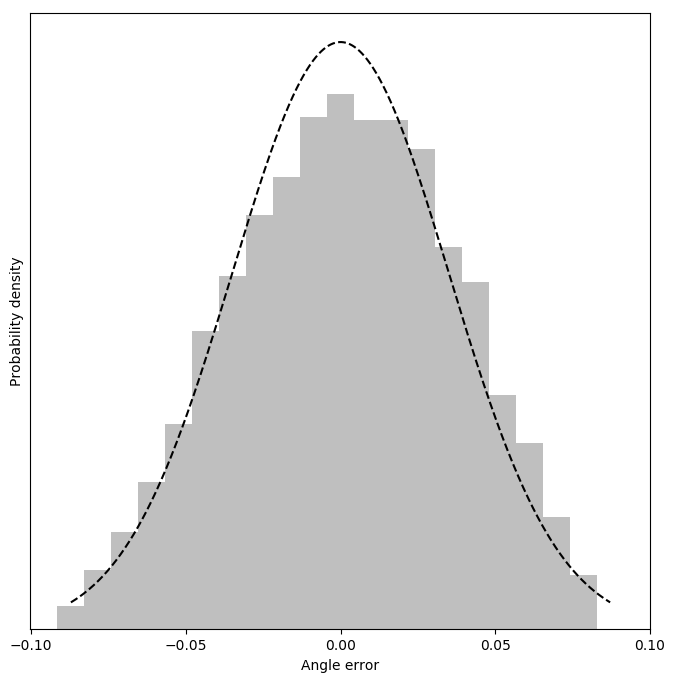
\includegraphics[width=\linewidth]{uncertainty}
  \end{minipage}
  \begin{minipage}{.5\textwidth}
    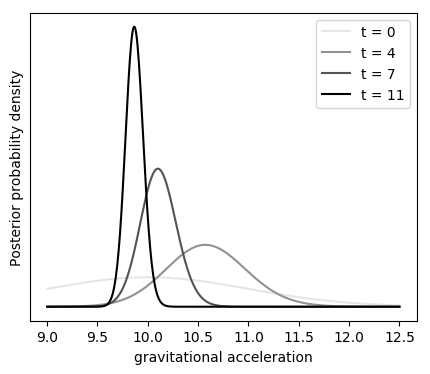
\includegraphics[width=0.97\linewidth]{posteriors}
  \end{minipage}
  \caption{Left: numerical forward propagation of time uncertainties through the pendulum's model. Dashed line is the density function of the Gaussian used to model the uncertainty in the probabilistic model. Right: Sequence of posteriors densities after observing $n=0, 3, 6, 9$ data points from light to dark, the lightest and darkest being prior and posterior density. }
  \label{uncertainty-posteriors}
\end{figure}


\begin{proof}
  We first prove that the solution $x(t)$ of the initial value problem is bounded, which is a stronger property than property i). We start by defining the Hamiltonian
  \begin{equation*}
    H(x, x') = \frac12 x'^2 - \frac{g}{l}\cos(x).
  \end{equation*}
  By simple calculation, one can show that $H$ is constant along the solution of the initial value problem. Since the initial values are $x_0 \in (0, \pi/2)$ and $x_0' = 0$, we have $H(x(t), x'(t)) = -\frac{g}{l}\cos(x_0) \in (-\frac{g}{l}, 0)$ for all $t > 0$. Assuming that $x(t)$ is not bounded, since $x$ is continuous and $x_0 \le \pi/2$, there is a time $t^\star$ such that $x(t^\star) = \pi$, giving
  \begin{equation*}
    H(x(t^\star), x'(t^\star)) = \frac12 x'(t^\star)^2 - \frac{g}{l}cos(x(t^\star)) \ge -\frac{g}{l}\cos(\pi) = \frac{g}{l} > 0.
  \end{equation*}
  This contradicts $H(x(t), x'(t)) = H(x_0, x'_0) \in (\frac{g}{l}, 0)$.Thus the solution of the initial value problem is bounded and so is $\mathcal{G}$, proving i).
  Furthermore, we know that the solution of the initial value problem is continuously differentiable with respect to $g$, it is thus locally Lipschitz continuous everywhere, and so is $\mathcal{G}$, thus completing the proof.
\end{proof}


%%% Local Variables:
%%% mode: latex
%%% TeX-master: "Thesis"
%%% End:
